
 		\begin{figure}
 			\centering
 			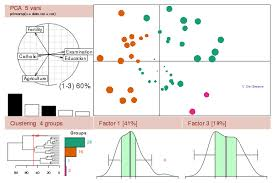
\includegraphics[width=0.97\linewidth]{CRAN}
 			\caption{Comprehensive R Archive Network}
 			
 		\end{figure}
 		
 		

 		\frametitle{R Packages}
 		
 		\begin{itemize}
 			\item ``10 R packages I wish I knew about earlier" - Drew Conway (Yhat.com, February 2013)
 			\bigskip \item ``The HadleyVerse" - Hadley Wickham
 			\begin{itemize}
 				
 				\item  ggplot2, dplyr, reshape, lubridate, stringr
 				
 				\item  With Romain Francois, Dianne Cook and Garret Grolemund.
 			\end{itemize}
 			\bigskip
 			\item Dr Brendan Haplin (UL): lme4 ,TraMineR, Gelman's arm, MASS, foreign. 
 			\bigskip
 			\item Shiny - Web Applications with \texttt{R}
 		\end{itemize}

 		
 		
 		
 		Some examples of packages are Actuar, written for actuarial science, and
 		QRMlib, which complements the Quantitative Risk Management The command library()
 		lists all the available packages. 
 		
 		To load a particular package, for example MASS, we would
 		write
 		library(MASS)
 		
<p>

 		
 		\frametitle{Packages}
 		\begin{itemize}
 			\item The CRAN package repository features 6107 available packages. 
 			\item Packages contain
 			various functions and data sets for numerous purposes, e.g.
 			\textbf{\textit{ggplot2}} package, \textbf{\textit{AER}} package, \textbf{\textit{survival}} package, etc.
 			\item Some packages are part of the basic installation. Others can be
 			downloaded from CRAN.
 			\item To access all of the functions and data sets in a particular package,
 			it must be loaded into the workspace. 
 			\item For example, to load the
 			\textbf{\textit{ggplot2}} package:
 		\end{itemize}
 		\begin{framed}
 			\begin{verbatim}
 			install.packages(ggplot2)
 			library(ggplot2)
 			\end{verbatim}
 		\end{framed}
<p>

 		\frametitle{4.2 Using and Installing packages}
 		\begin{itemize}
 			\item Many packages come with R. To use them in an R session, you need to load the package, as
 			previously demonstrated.
 			\item Some packages are not automatically installed when you install R but they need to be downloaded
 			and installed individually. 
 			\item We must first install them using the install.packages()
 			function, which typically downloads the package from CRAN and installs it for use. (follow the
 			instructions as indicated).
 		\end{itemize}
<p>

 		\begin{framed}
 			\begin{verbatim}
 			install.packages("ggplot2")
 			install.packages("qcc")
 			install.packages("sqldf")
 			install.packages("RMongo")
 			install.packages("randomforest")
 			\end{verbatim}
 		\end{framed}
 		
<p>

 		\frametitle{4.2.1 Version of R}
 		Many packages will require you to have the most recent version of R and also other packages.
 		It is a good idea to update regularly.

<p>

 		5 Data Creation, Data Entry, Data Import and Export

<p>


 		\frametitle{5.1 The \texttt{c()} command}
 		To create a simple data set, known as a vector, we use the c() command to create the vector.
 		\begin{framed}
 			\begin{verbatim}
 			> Y=c(1,2,4,8,16 ) #create a data vector with specified elements
 			> Y
 			[1] 1 2 4 8 16
 			
 			\end{verbatim}
 		\end{framed}
 		
<p>

 		\frametitle{Vectors}
 		\begin{framed}
 			\begin{verbatim}
 			### Vector of Numeric Values
 			Numvec = c(10,13,15,19,25);
 			## Vector of Character Values
 			Charvec = c("LouLou","Oscar","Rasher");
 			
 			## Vector of Logical Values
 			Charvec = c(TRUE,TRUE,FALSE,TRUE);
 			\end{verbatim}
 		\end{framed}
<p>

 		\frametitle{Vectors}	
 		Vectors can be bound together either by row or by column.
 		\begin{framed}
 			\begin{verbatim}
 			> X=1:3; Y=4:6
 			> cbind(X,Y)
 			X Y
 			[1,] 1 4
 			[2,] 2 5
 			[3,] 3 6
 			>
 			> rbind(X,Y)
 			[,1] [,2] [,3]
 			X 1 2 3
 			Y 4 5 6
 			\end{verbatim}
 		\end{framed}
<p>

 		\frametitle{5.2 The scan() command}
 		\begin{itemize}
 			\item	The \texttt{scan()} function is a useful method of inputting data quickly. 
 			\item You can use to quickly copy
 			and paste values into the \texttt{R} environment. It is best used in the manner as described in the
 			following example. 
 			\item Create a variable ”X” and use the \texttt{scan()} function to populate it with
 			values. 
 			\item Type in a value, and then press return. Once you have entered all the values, press
 			return again to return to normal operation.
 		\end{itemize}
<p>


 		\begin{verbatim}
 		> X=scan()
 		1: 4
 		2: 5
 		3: 5
 		4: 6
 		5:
 		Read 4 items
 		\end{verbatim}
 		Remark: Try the edit() command on object X.

<p>

 		5.2.1 Characters with the scan() command
 		The scan() command can also be used forinputting character data.
 		> Y=scan(what=" ")
 		1: LouLou
 		2: Oscar
 		3: Rasher
 		4:
 		Read 3 items
 		> Y
 		[1] "LouLou" "Oscar" "Rasher"
 	\end{frame}
 	%==============================================================================================%
 	\begin{frame}[fragile]
 		5.3 Using the data editor
 		5.4 Spreadsheet Interface
 		R provides a spreadsheet interface for editing the values of existing data sets. We use the
 		command \texttt{data.entry()}, and name of the data object as the argument. (Also try out the
 		fix() command)
 		\begin{framed}
 			\begin{verbatim}
 			> data.entry(X) # Edit the data set and exit interface
 			> X
 			\end{verbatim}
 		\end{framed}
 		

 	
 	
